%%%%%%%%%%%%%%%%%%%%%%%%%%%%%%%%%%%%%%%%%%%%%%%%%%%%%%%%%%%%%%%%%%%%%%%%%%%%%%%%
%2345678901234567890123456789012345678901234567890123456789012345678901234567890
%        1         2         3         4         5         6         7         8

\documentclass[letterpaper, 10 pt, conference]{ieeeconf}  % Comment this line out
                                                          % if you need a4paper
%\documentclass[a4paper, 10pt, conference]{ieeeconf}      % Use this line for a4
                                                          % paper

\IEEEoverridecommandlockouts                              % This command is only
                                                          % needed if you want to
                                                          % use the \thanks command
\overrideIEEEmargins
% See the \addtolength command later in the file to balance the column lengths
% on the last page of the document



% The following packages can be found on http:\\www.ctan.org
%\usepackage{graphics} % for pdf, bitmapped graphics files
%\usepackage{epsfig} % for postscript graphics files
%\usepackage{mathptmx} % assumes new font selection scheme installed
%\usepackage{times} % assumes new font selection scheme installed
%\usepackage{amsmath} % assumes amsmath package installed
%\usepackage{amssymb}  % assumes amsmath package installed


\usepackage[utf8]{inputenc}
\usepackage{graphicx}
\usepackage{endnotes}

\usepackage{mathtools}
\DeclarePairedDelimiter\ceil{\lceil}{\rceil}
\DeclarePairedDelimiter\floor{\lfloor}{\rfloor}

\usepackage{algorithm}
\usepackage{algpseudocode}
\usepackage{listings}
\usepackage{color}

\definecolor{miverde}{rgb}{0,0.6,0}
\definecolor{migris}{rgb}{0.5,0.5,0.5}
\definecolor{mimalva}{rgb}{0.58,0,0.82}

\lstset{ %
  backgroundcolor=\color{white},   % Indica el color de fondo; necesita que se añada \usepackage{color} o \usepackage{xcolor}
  basicstyle=\footnotesize,        % Fija el tamaño del tipo de letra utilizado para el código
  breakatwhitespace=false,         % Activarlo para que los saltos automáticos solo se apliquen en los espacios en blanco
  breaklines=true,                 % Activa el salto de línea automático
  captionpos=b,                    % Establece la posición de la leyenda del cuadro de código
  commentstyle=\color{miverde},    % Estilo de los comentarios
  deletekeywords={...},            % Si se quiere eliminar palabras clave del lenguaje
  escapeinside={\%*}{*)},          % Si quieres incorporar LaTeX dentro del propio código
  extendedchars=true,              % Permite utilizar caracteres extendidos no-ASCII; solo funciona para codificaciones de 8-bits; para UTF-8 no funciona. En xelatex necesita estar a true para que funcione.
  frame=single,	                   % Añade un marco al código
  keepspaces=true,                 % Mantiene los espacios en el texto. Es útil para mantener la indentación del código(puede necesitar columns=flexible).
  keywordstyle=\color{blue},       % estilo de las palabras clave
  language=Pascal,                 % El lenguaje del código
  otherkeywords={*,...},           % Si se quieren añadir otras palabras clave al lenguaje
  numbers=none,                    % Posición de los números de línea (none, left, right).
  numbersep=5pt,                   % Distancia de los números de línea al código
  numberstyle=\small\color{migris}, % Estilo para los números de línea
  rulecolor=\color{black},         % Si no se activa, el color del marco puede cambiar en los saltos de línea entre textos que sea de otro color, por ejemplo, los comentarios, que están en verde en este ejemplo
  showstringspaces=false,          % subraya solamente los espacios que estén en una cadena de esto
  stepnumber=2,                    % Muestra solamente los números de línea que corresponden a cada salto. En este caso: 1,3,5,...
  stringstyle=\color{mimalva},     % Estilo de las cadenas de texto
  tabsize=2,	                   % Establece el salto de las tabulaciones a 2 espacios
  title=\lstname                   % muestra el nombre de los ficheros incluidos al utilizar \lstinputlisting; también se puede utilizar en el parámetro caption
}

\title{\LARGE \bf
IIC 3633 - Recommender Systems\\
Homework Assignment 1
}

% \author{ \parbox{3 in}{\centering Huibert Kwakernaak*
%         \thanks{*Use the $\backslash$thanks command to put information here}\\
%         Faculty of Electrical Engineering, Mathematics and Computer Science\\
%         University of Twente\\
%         7500 AE Enschede, The Netherlands\\
%         {\tt\small h.kwakernaak@autsubmit.com}}
%         \hspace*{ 0.5 in}
%         \parbox{3 in}{ \centering Pradeep Misra**
%         \thanks{**The footnote marks may be inserted manually}\\
%         Department of Electrical Engineering \\
%         Wright State University\\
%         Dayton, OH 45435, USA\\
%         {\tt\small pmisra@cs.wright.edu}}
% %}

\centering \author{ Paula Navarrete Campos\\
        Department of Industrial and Systems Engineering\\
        School of Engineering\\
        {\tt\small pcnavarr@uc.cl}}

\noaffiliation

\begin{document}



\maketitle
\thispagestyle{empty}
\pagestyle{empty}


%%%%%%%%%%%%%%%%%%%%%%%%%%%%%%%%%%%%%%%%%%%%%%%%%%%%%%%%%%%%%%%%%%%%%%%%%%%%%%%%

%%%%%%%%%%%%%%%%%%%%%%%%%%%%%%%%%%%%%%%%%%%%%%%%%%%%%%%%%%%%%%%%%%%%%%%%%%%%%%%%

This work develops a recommendation system for the beer industry based on Collaborative Filtering. Schafer et al. (2007) \cite{c1} and Koren et al. (2009) \cite{c3} disentangle key concepts on collaborative filtering (CF), exposing its main uses, algorithms and design decisions regarding rating systems and ratings acquisition. 
There is some common grounded theory to take into account when designing and developing a recommender system, mainly regarding approach, data nature and purpose of the software.

\section{Introduction and Objectives}

Collaborative Filtering is the process of filtering or evaluating items using the opinions of other people, taking its roots in the old human behavior of sharing opinions. There are some key concepts in this approach to making recommendations. 

\begin{itemize}

    \item \textit{Rating} consists on associating two things, user and item, usually through some value. This can be visualized through a \textit{ratings matrix}, where each row represents a user and each column represents an item, with the intersection being the value of the rating (the absence of value means that the user has not evaluated the item). The measure of the rating can be a scalar (numerical measure), binary (as decisions type agree/disagee, like/dislike) or unary (for example, if the user saw the item, or if he rated it positively).

    \item \textit{User} corresponds to the person who provides ratings to the system or who uses it to receive information.
    
    \item Collaborative filtering systems produce recommendations or predictions for a user and at least one item, which can be anything that can be ``evaluated'' by a human.

\end{itemize}\includegraphics[scale=1.5]{lion-logo}

\section{Exploratory Data Analysis}

Breve análisis de los datos que incluya, al menos, estadísticas
de los usuarios, densidad del dataset y gráficos de distribución (usuario/ítem e ítems/usuario).
responder si es explicit or implicit feedback feedback. Característica de la matriz, es sparce o dense? qué método han sugerido los papers leidos que funcionará mejor?

\begin{enumerate}
    \item \textbf{Density}
    
    
        \begin{figure}[h]
            
            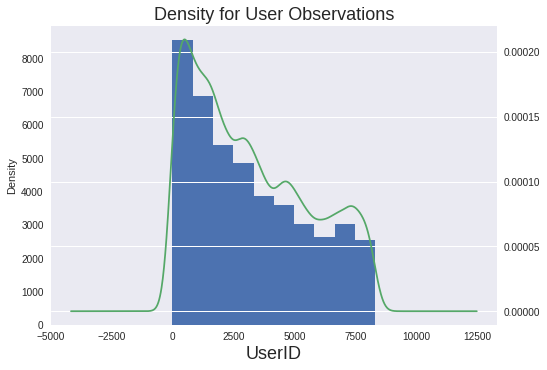
\includegraphics[scale=0.4]{userID_hist-kde.png}
            \centering
            \caption{Density for user rating observations}
            % Figure reference: \ref{fig:fig-name}
            % Figure page reference:  \pageref{fig-name} 
            \label{fig:user-density}
            
        \end{figure}
        
        The shape of the figure \ref{fig:user-density} is congruent with the tendency to have less users in the beginnig (the so-called early adopters) giving lots of ratings and helping the system to learn, and afterwads, a lot of new users giving a lot of less reviews. The same can be chequed out analogously for the items.

 

        
        \begin{figure}[h]
            
            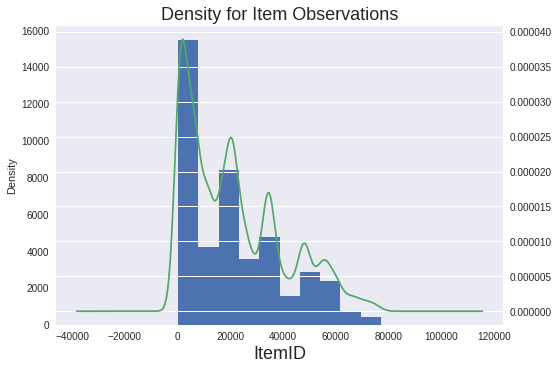
\includegraphics[scale=0.4]{ItemID_hist-kde.png}
            \centering
            \caption{Density for item rating observations}
            % Figure reference: \ref{fig:fig-name}
            % Figure page reference:  \pageref{fig-name} 
            \label{fig:item-density}
            
        \end{figure}
        
        It is interesting what the figure \ref{fig:item-density} shows. We can see a sort of different waves, characterized by a peak of ratings for some items, but a comparable bigger tail of items rated comparatively less. This may suggest that new items were introduced in 4 to 5 waves along time, where we initial introductions brought several more reviews per item introduced than the later, making sense with the previous analysis of users.
    
    \item \textbf{Distribution}
    
         \begin{figure}[h]
            
            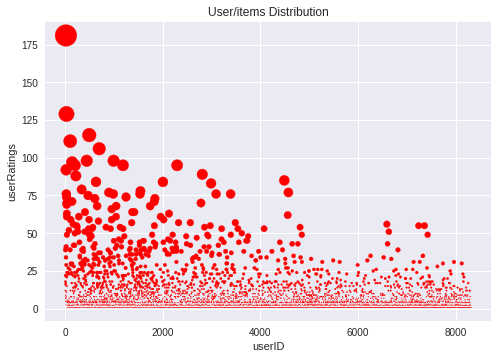
\includegraphics[scale=0.4]{User-item_distribution.png}
            \centering
            \caption{Distribution for user itemRatings}
            % Figure reference: \ref{fig:fig-name}
            % Figure page reference:  \pageref{fig-name} 
            \label{fig:user-distribution}
            
        \end{figure}
        
        \begin{figure}[h]
            
            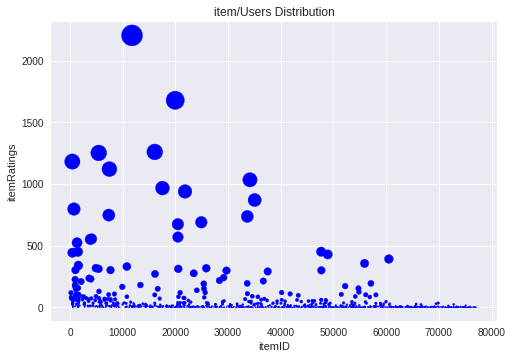
\includegraphics[scale=0.4]{Item-user_distribution.png}
            \centering
            \caption{Distribution for item userRatings}
            % Figure reference: \ref{fig:fig-name}
            % Figure page reference:  \pageref{fig-name} 
            \label{fig:item-distribution}
            
        \end{figure}
    
    
\end{enumerate}

\section{Experimental Design}

Describir de forma breve la metodología de los experimentos: Qué
se hizo con los datos y por qué (particiones, cross-validation, etc.), qué métodos se usaron y por
qué.
calcular también tiempo de ejecución, procesamiento y memoria requeridos.
\begin{enumerate}

    \item \textbf{UserKnn:} This algorithm interprets similar users as neighbors, if the user $n$ is similar to the user $u$, then $n$ is a neighbor of $u$. It generates a prediction for an item $i$ by analyzing the ratings for $i$ from the users in the neighborhood of $u$. Where:
    
    \begin{equation}
        pred(u,i)=\Bar{r}+ \frac{\displaystyle \sum_{n \subset N(u)}uSim(u,n)*(r_{ni}-\Bar{r}_{n})}{\displaystyle \sum_{n \subset N(u)}uSim(u,n)}
    \end{equation}
    Donde $N(u)$ son los vecinos de $u$ y corresponde a la predicción para item i que evalúa los ratings para ese i de los vecinos de u. Esta fomulación corrige las variaciones en la escala de rating y pondera cada uno por las similaridades de cada usuario con u (el término inferior corresponde a la normalización del resultado).
    
    Una forma de medir la similaridad expresada en la formulación anterior es a través de la correlación de Pearson, donde: 
    
    \begin{equation}
        uSim(u,n)= \frac{ \sum_{i \subset CR(u,n)}(r_{ui}-\Bar{r}_{u})(r_{ni}-\Bar{r}_{n})}{ \displaystyle \sqrt{\displaystyle \sum_{i \subset CR_{(u,n)}}(r_{ui}-\Bar{r}_{u})^2}  \sqrt{\displaystyle \sum_{i \subset CR_{(u,n)}}(r_{ni}-\Bar{r}_{n})^2} }
    \end{equation}
    
    Where $CR_{(u, n)} $ are the coevaluated itemes between $ u $ and $ n $ and represents the similarity between the user $ u $ with user  $ n $ and $ \in [-1.0, 1.0] $, where $ 1.0 $ corresponds to a perfect similarity and $ -1.0 $ to its complement, in this context, we can choose only positive correlations to improve the prediction. This formulation analyzes similarities in ratings for items evaluated together with $ i $ (corrating).
    
    Although $UserKnn$ captures how recommendations are arranged and can detect complex patterns, as the data is sparce, it does not achieve general consensus regarding an item and pairs of users with few corratings are prone to throw biased correlations that can dominate the user's neighborhood in question.
    
    The algorithm can be implemented including all the users of the set as neighbors of each user, although by limiting it to the closest $k$ neighbors to each user improves its accuracy and efficiency. The challenge is to choose a well suited $k$ for the dataset. Even so, its implementation is expensive since it requires comparing each user with the complete set, so the time and memory for processing do not scale well as users and ratings increase. 
    
    
    \item \textbf{ItemKnn:}, estimaer mejor k
    
    Item-based Nearest Neighbor (IBNN): Corresponden a transponer el problema anterior, mientras que los algoritmos user-based generan predicciones basadas en similaridades entre usuarios, los item-based lo hacen basándose en similaridades entre items, es decir, la predicción para un item se basa en ratings para items similares. Así, una predicción para un usuario u de un item i puede ser representada como la composición de sumas ponderadas de ratings del mismo usuario para los items mas similares de i (análogamente a la derivación (4)).
    
    \begin{equation}
        pred(u,i)=\Bar{r}+ \frac{\displaystyle \sum_{n \subset RI(u)}iSim(i,j)*r_{ui}}{\displaystyle \sum_{n \subset RI(u)}iSim(i,j)}
    \end{equation}
    Donde $RI(u)$ corresponde a los itemes evaluados por $u$.
    
    Como los datos con que se compone la predicción están dados por todos los correspondientes al mismo usuario, no es necesario centrar la suma ponderada como en el caso anterior. Análogamente, itemSim() corresponde a la medida de similaridad entre los itemes i y j. La métrica de similaridad mas popular y precisa para calcular esta similaridad es la del coseno subjacente ajustado que se muestra a continuación: 
     \begin{equation}
        iSim(u,n)=\frac{\displaystyle \sum_{u \subset RB_{i,j}}(r_{ui}-\Bar{r}_{u})(r_{uj}-\Bar{r}_{u})}{ \sqrt{\displaystyle \sum_{u \subset RB_{i,j}}(r_{ui}-\Bar{r}_{u})^2}  \sqrt{\displaystyle \sum_{u \subset RB_{i,j}}(r_{uj}-\Bar{r}_{u})^2} }
    \end{equation}
    
    Donde el set $RB_{i,j}$ corresponde al set de usuarios que han dado rating tanto a $i$ como a $j$. Aunque hay evidencia de que IBNN es más preciso que UBNN, de todas formas el tamaño del modelo crece cuadráticamente con el número de items. Hay diferentes técnicas para mejorar el uso de memoria, como limitar el procesamiento hasta k corratings o retener solo las n mejores correlaciones para cada item (esto puede provocar que los itemes correlacionados con los ratings del usuario no contengan el item objetivo)
    
    \item \textbf{SlopeOne:},
    \item \textbf{SVD:}.
    \item \textbf{ALS o ALScg:} este modelo lo puede usar para la tarea de ranking. Si tiene problemas con pyreclab, puede usar la biblioteca implicit1.
\end{enumerate}


\section{Results}

El informe debe tener una tabla donde las filas presentan
los métodos y las columnas las metricas RMSE, MAE, MAP@10 y nDCG@10. Presente en esta tabla cada método sólo una vez. Si el método tiene parámetros, presente la versión del método con los parámetros que le dieron mejores resultados.

\section{Results}

Describir los resultados obtenidos. Además deben comparar y
analizar los diferentes métodos respecto a, al menos, su implementación (dificultades y otros),
tiempo de ejecución, procesamiento y memoria requeridos, y métricas de rendimiento (RMSE y
nDCG).

\section{Sensitivity Analysis (Discussion?)}

Explicar el efecto de los diferentes parámetros
que escogieron en los resultados obtenidos.

\section{Conclusion}

Conclusiones a las que se llegó luego de realizar la tarea.


\addtolength{\textheight}{-12cm}   % This command serves to balance the column lengths
                                  % on the last page of the document manually. It shortens
                                  % the textheight of the last page by a suitable amount.
                                  % This command does not take effect until the next page
                                  % so it should come on the page before the last. Make
                                  % sure that you do not shorten the textheight too much.


\begin{thebibliography}{99}

\bibitem{c1} Schafer, J. B., Frankowski, D., Herlocker, J., & Sen, S. (2007). Collaborative filtering recommender systems. In The adaptive web (pp. 291-324). Springer Berlin Heidelberg.

\bibitem{c2} How not to sort by Average Rating, Evan Miller Blog

\bibitem{c3} Koren, Y., Bell, R., & Volinsky, C. (2009). Matrix factorization techniques for recommender systems. Computer IEEE Magazine, 42(8), 30–37.

\bibitem{c4} Hu, Y., Koren, Y., & Volinsky, C. (2008, December). Collaborative filtering for implicit feedback datasets. In Data Mining, 2008. ICDM’08. Eighth IEEE International Conference on (pp. 263–272). IEEE.


\bibitem{c5} L. Van der Maaten and G. Hinton. Visualizing data using t-sne. Journal of Machine Learning Research, 9(2579-2605):85, 2008.








\end{thebibliography}




\end{document}
